\section{Practice}
\label{sec:experiments}

This section will provide the implementation details of the theory part (Section \ref{sec:theory}). The algorithm is implemented in C ++ and makes use of the CGAL library (\url{https://www.cgal.org}). Then, given the implementation, a preliminary experimental setup will be introduced. The experimental setup will include some basic test polygons to check the correct execution of the algorithm. Additionally, we will observe the behaviour of the algorithm and propose preparatory experiments for the second phase of the thesis.
% As such, we will devise an algorithm for optimising the positions of the guards inside the given Art Gallery polygon. 
% The algorithm is coded in C ++ with the use of the CGAL library (\url{https://www.cgal.org}).
\subsection{Implementation}
In Section \ref{sec:theory} we devised formula \ref{eq:l} for computing the gradient of one guard and the reflex vertices it can see. This section will show the implementation and use of the formula to iteratively optimise a guard's position. 

The implementation takes a polygon and a guard with an arbitrary position as input. The main idea of the algorithm is that the position of the guard is continuously improved until an optimum is found. That is, until the computed gradient does not change the position of the guard anymore.
It can happen that the gradient computes an optimised position of the guard outside the polygon. In that case, the guard is placed and subsequently moved on the polygon boundary. The pseudo-code can be found in Algorithm \ref{alg:1g}.

\begin{algorithm}[H]
    \begin{algorithmic}[1]
    \caption{Position Optimisation for One Guard}
    \label{alg:1g}

    \State{\textbf{Input:} polygon $P$, guard $g(x, y)$}
    \State{\textbf{Output:} optimised position $g'(x', y')$ of the guard}
    \State{}
    % \For{\textbf{each} guard $p(x, y)$}
    \State{\textit{cur\_guard\_position} $\gets g(x, y)$}

    \While{\textit{prev\_guard\_position} $\neq$ \textit{cur\_guard\_position} \textbf{and} the whole polygon is not seen} %\Comment{continue as long as there are no more improvements in the guard's position}
        % \State{compute \textit{visibility\_region} of $p$}
        \State{compute $\bigtriangledown f(\textit{cur\_guard\_position})$}
        \State{\textit{prev\_guard\_position} $\gets$ \textit{cur\_guard\_position}}
        \State{\textit{cur\_guard\_position} $\gets \textit{prev\_guard\_position} + l\bigtriangledown f$}

        \If{\textit{cur\_guard\_position} is outside the polygon}
            \State{place \textit{cur\_guard\_position} on polygon boundary}
        \EndIf
    \EndWhile
    \State{$g'(x', y') \gets \textit{cur\_guard\_position}$}
    % \EndFor
    \State \Return $g'$
    \end{algorithmic}
\end{algorithm}

The implementation has been tested with one guard and multiple input polygons. The polygons target specific use- or edge-cases. These cases will be built upon when expanding the implementation to multiple guards. The current input polygons are:

% are the irrational guard polygon (Figure \ref{fig:p}), a star-shaped polygon (Subfigure \ref{fig:star}), a comb-shaped polygon (Subfigure \ref{fig:comb}), an arrow head (Subfigure \ref{fig:concave}) and an arbitrary polygon (Subfigure \ref{fig:random}). Each of them will be used for testing various aspects of the algorithm as follows:

\begin{itemize}
    \item the \textbf{star polygon} (Subfigure \ref{fig:star}) tests whether guards can do basic moves from the inside the polygon to the centre of it. The star polygon can be fully seen by 1 guard.
    \item the \textbf{arrowhead polygon} (Subfigure \ref{fig:concave}) tests the movement of guard to optimality on the boundary of the polygon. The arrowhead polygon can be fully seen by 1 guard.
    \item the \textbf{comb polygon} (Subfigure \ref{fig:comb}) tests the algorithm with multiple guards. The comb polygon can be fully guarded by 4 points, each of them placed in each one of the spikes.
    \item the \textbf{arbitrary polygon} (Subfigure \ref{fig:random}) combines the previously mentioned cases. The arbitrary polygon can be fully seen by 3 guards.
    \item the \textbf{irrational guards polygon} (Figure \ref{fig:p}) combines the previously mentioned cases. The irrational guards polygon can be fully seen by either 3 guards with irrational coordinates, or 4 guards with rational coordinates.
\end{itemize}

\begin{figure}[h!]
    \centering
    \begin{subfigure}{0.45\textwidth}
        \centering
        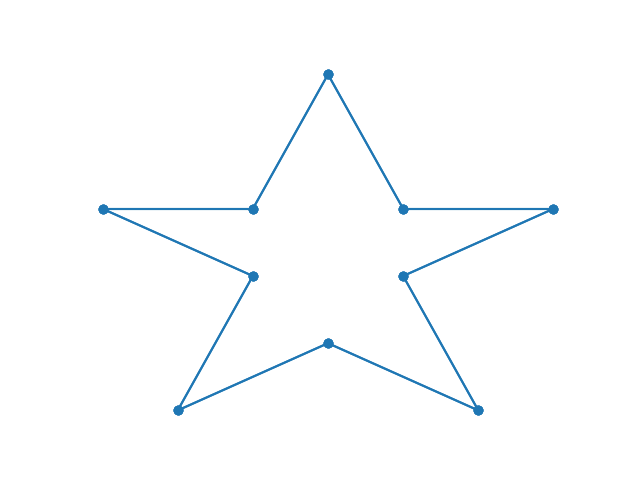
\includegraphics[width = \textwidth]{pentagram.png}
        \caption{Star test input polygon.}
        \label{fig:star}
    \end{subfigure}
    \begin{subfigure}{0.45\textwidth}
        \centering
        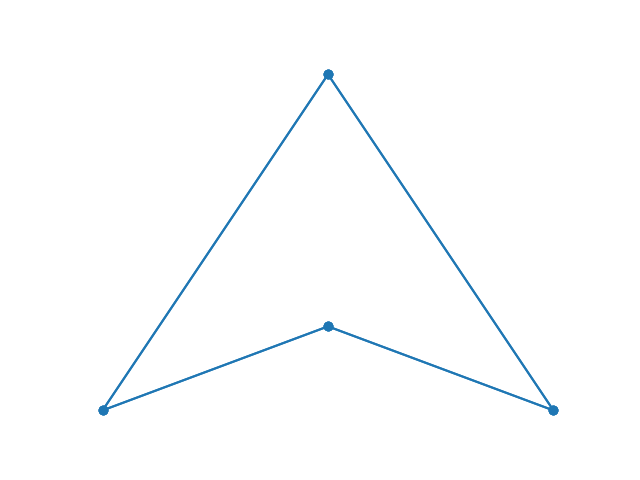
\includegraphics[width = \textwidth]{concave_triangle.png}
        \caption{Arrowhead test input polygon.}
        \label{fig:concave}
    \end{subfigure}
    \begin{subfigure}{0.45\textwidth}
        \centering
        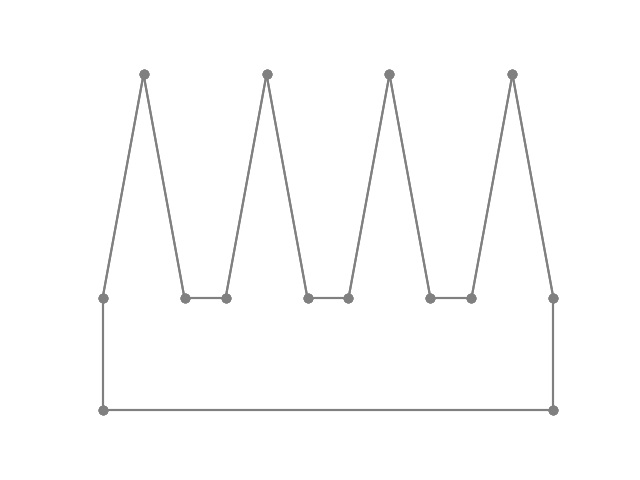
\includegraphics[width = \textwidth]{comb.png}
        \caption{Comb test input polygon.}
        \label{fig:comb}
    \end{subfigure}
    \begin{subfigure}{0.45\textwidth}
        \centering
        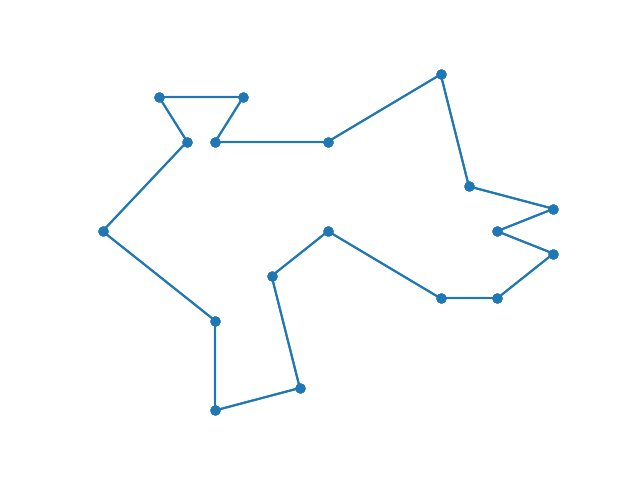
\includegraphics[width = \textwidth]{random.png}
        \caption{Arbitrary test input polygon.}
        \label{fig:random}
    \end{subfigure}
    \caption{Input polygons used for testing the algorithm.}
\end{figure}
% Timetable and planning What will you do with the remainder of my thesis? Give an approximate estimation/timetable for what you will do and when you will be done.
\subsection{Preliminary Results}
This subsection will provide some exploratory results based on the current implementation. The implementation is tested on the five previously mentioned input polygons and an arbitrarily placed guard. Firstly, we will validate the correct execution of the algorithm by checking whether the positions of guards is optimised as expected. Then, we will explore how different learning rates influence the results on different types of polygons. Lastly, we will aim to smoothen out the large noisy jumps in the gradient descent computation by using momentum \cite{goodfelow2016deep}. In this way, we will create an ``inertia'' effect by extending the gradient descent algorithm with a moving average of previously computed states.

\subsubsection{Checking Correct Execution}
We will first validate that the implemented algorithm runs correctly. Thus, we expect that for the polygons that can be guarded by only one point, the algorithm will find an optimal position of the guard. For polygons that require multiple guards, we expect that the algorithm will either settle in local maxima, or will jump between local maxima depending on the learning rate.

The algorithm is run with a learning rate of 0.2. This value was chosen as we expect it to be big enough to find an optimum position in a reasonable runtime. It should also small enough to observe a smooth, relevant transition in the guard's position.

The experiments have a 1-minute run timeout. This amount of time was chosen in order to build some intuition related to the speed of the algorithm. Namely, we expect that the algorithm would be fast for small input polygons. That is the case with the star and the arrowhead polygons in Subfigures \ref{fig:star_gradient} and \ref{fig:concave_gradient}. There, the final guard positions are optimally found within 1 minute. From this position, the polygons are fully seen.


\begin{figure}[h!]
    \centering
    \begin{subfigure}{0.45\textwidth}
        \centering
        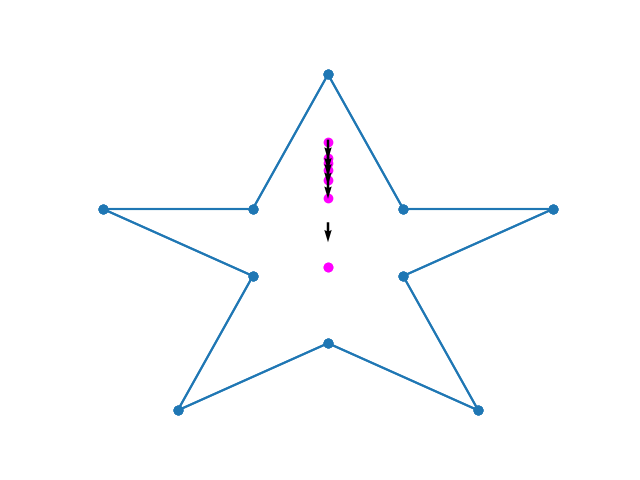
\includegraphics[width = \textwidth]{experiments/pentagram_gradient.png}
        \caption{Star polygon gradient run example.}
        \label{fig:star_gradient}
    \end{subfigure}
    \begin{subfigure}{0.45\textwidth}
        \centering
        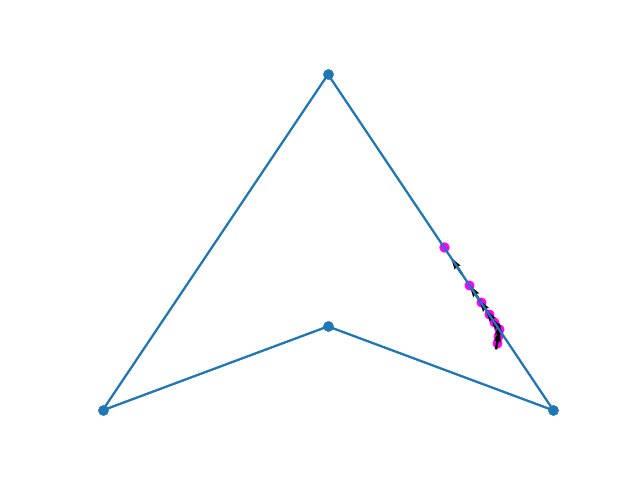
\includegraphics[width = \textwidth]{experiments/concave_triangle_gradient.png}
        \caption{Arrowhead polygon gradient run example.}
        \label{fig:concave_gradient}
    \end{subfigure}
    \begin{subfigure}{0.45\textwidth}
        \centering
        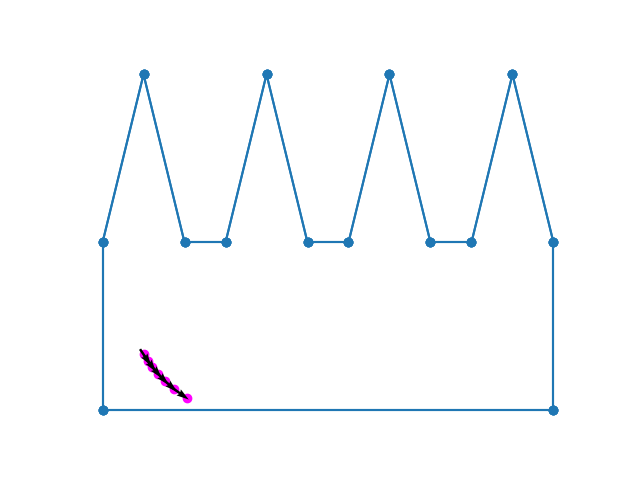
\includegraphics[width = \textwidth]{experiments/comb_gradient.png}
        \caption{Comb polygon gradient run example.}
        \label{fig:comb_gradient}
    \end{subfigure}
    \begin{subfigure}{0.45\textwidth}
        \centering
        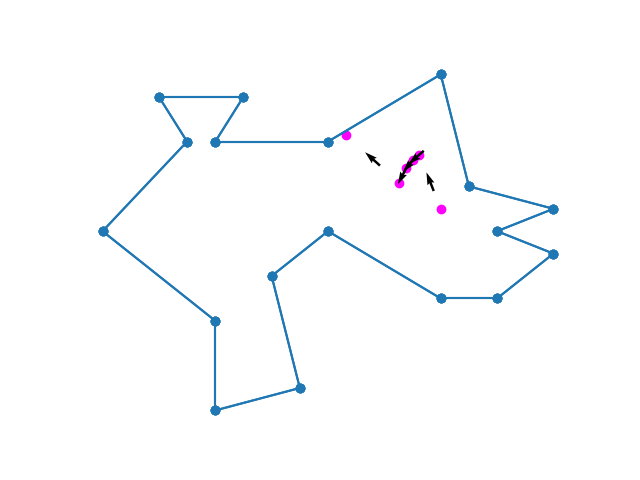
\includegraphics[width = \textwidth]{experiments/random_gradient.png}
        \caption{Arbitrary polygon gradient run example.}
        \label{fig:random_gradient}
    \end{subfigure}
    \begin{subfigure}{\textwidth}
        \centering
        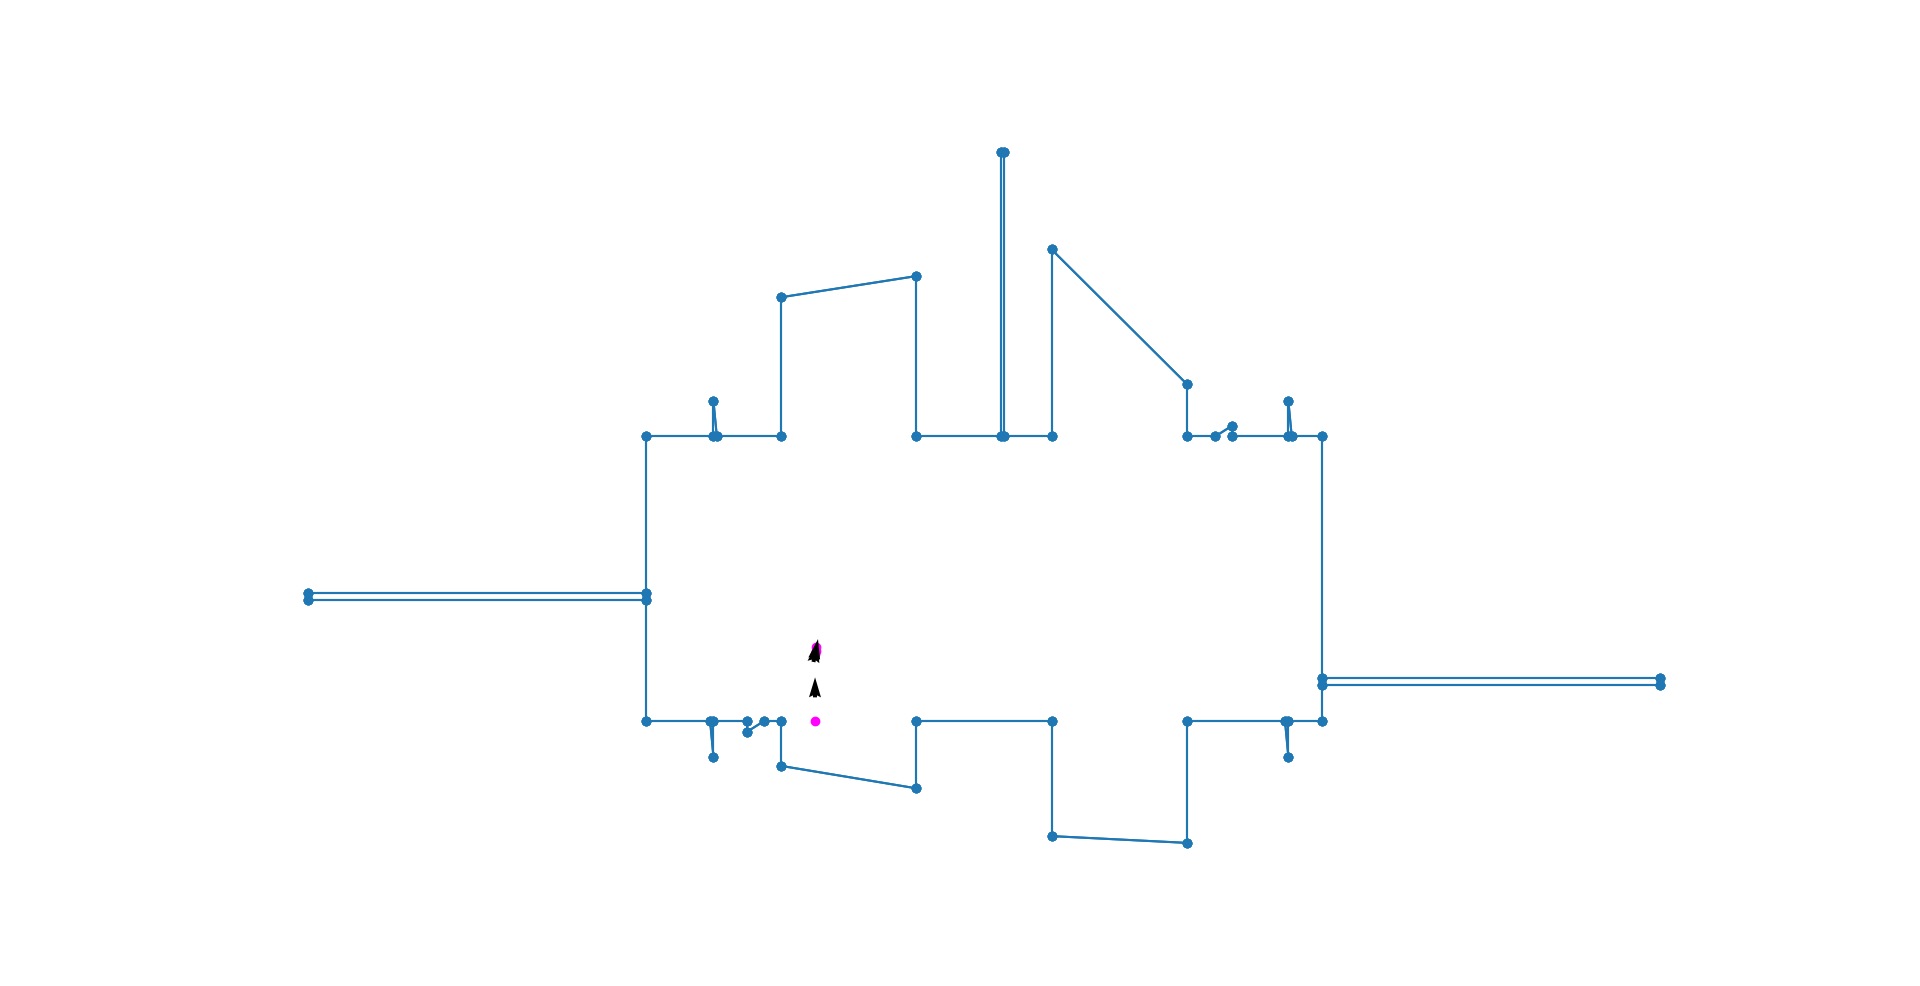
\includegraphics[width = \textwidth]{experiments/love_gradient.png}
        \caption{Irrational guard polygon gradient example.}
        \label{fig:love_gradient}
    \end{subfigure}
    \caption{Gradient descent examples with learning rate $\alpha = 0.2$ on the test polygons.}
    \label{fig:gradients}
\end{figure}

This is not the case with the rest of the three input polygons. Currently, the implementation slows down in this case as the algorithm progresses when computing the visibility region and the gradient of the guard. Nonetheless, the final position of the guard in Subfigures \ref{fig:comb_gradient}, \ref{fig:random_gradient} and \ref{fig:love_gradient} is the last computed position at timeout. Additionally, these polygons require multiple guards to be fully visible. For this reason, we expect that gradient descent would either settle in a local optimum, or would continuously jump between multiple local optima given a large enough learning rate.

In the case of the comb polygon (Subfigure \ref{fig:comb_gradient}), the tendency of the guard is to move towards the lower boundary of the polygon. This maximises the area observed by the guard, although the guard alone will not able to see all the spikes at once. 
When given a longer timeout, we expect that the algorithm would move the guard between the local optima below each of the spikes. 
% In the second part of this thesis, we aim at mitigating the slowdown issue. Then we will explore whether a jump between local optima happens indeed.

The arbitrary polygon (Subfigure \ref{fig:random_gradient}) shows similar behaviour in terms of moving between local optima. Initially the guard takes a large jump from its initial position to a more fine-tuned path. After a few smoother steps, it takes another large jump close to the boundary of the polygon. We account the large uneven jumps to the nature of the gradient descent technique. Its computation is based only on the current position, irregardless of previous states. For this reason, when the guard approaches a reflex vertex and gains more visibility behind it, the larger jump happens. We will explore and attempt to mitigate this aspect in later subsections.
% In order to explore this aspect, we will later look into how the jumps between local optima differ given the learning rate.

Lastly, the algorithm managed to take the least number of steps within the time limit in the irrational guard polygon (Subfigure \ref{fig:love_gradient}). That is expected, as it is also the largest polygon out of all the input ones. This polygon can also not be guarded by only 1 point. For this reason, we cannot gain informative observations about the performance of the algorithm for this particular polygon.
% So, we will explore in the next subsection how the algorithm performs when different learning rates are used. 
% Moreover, we will also examine how well our approximation gradient descent algorithm performs when compared to the exact irrational positions of the guards.

Thus, we cannot draw a clear conclusion in terms of how the algorithm performs when tested on polygons requiring more than 1 guard. Due to the 1-minute timeout, we cannot observe whether the guard position jumps between multiple local optima, or is able to settle in a local maximum. For this reason, we will explore in the next subsection whether different learning rates can offer more insight into this matter.

Then, in a later subsection, we will explore taking into account previous positions of a guard. As such, we will attempt to extend the gradient descent technique with momentum \cite{goodfelow2016deep}. This will result in a smoothened out trajectory of the guard.

% \newpage
\subsubsection{Different Learning Rates}
We will experiment with how increasing the learning rate would affect the outcome of the algorithm on the test polygons. Namely, we will test how increasing the learning rate from $\alpha = 0.2$ to $\alpha \in \{0.4, 0.65\}$ would affect the one-guard placement in the input polygons. As such, we chose the arrowhead and the arbitrary polygons as the two test cases. The former polygon requires only one guard for full visibility, so we expect to validate the faster convergence to optimality as the learning rate increases. On the other hand, the latter polygon requires more guards. In this case, we expect to observe more concretely how the algorithm behaves when there are multiple local optima. Figure \ref{fig:multiple_gradients} displays the results for exploring these aspects. 

\begin{figure}[h!]
    \centering
    \begin{subfigure}{0.45\textwidth}
        \centering
        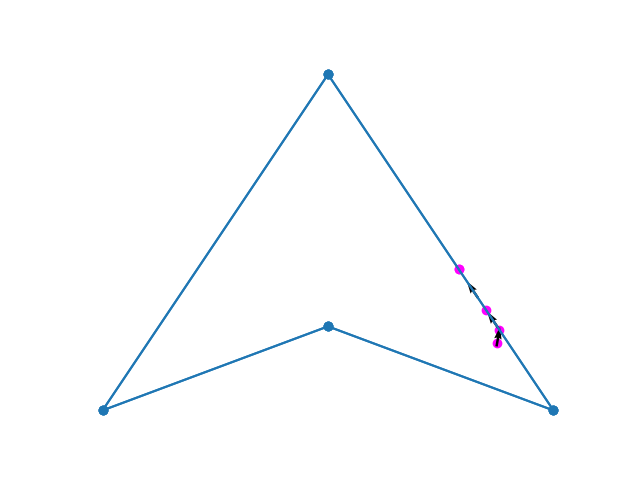
\includegraphics[width = \textwidth]{experiments/concave_triangle_gradient_045.png}
        \caption{Arrowhead polygon gradient with learning rate $\alpha = 0.45$ example}
        \label{fig:concave_gradient_045}
    \end{subfigure}
    \begin{subfigure}{0.45\textwidth}
        \centering
        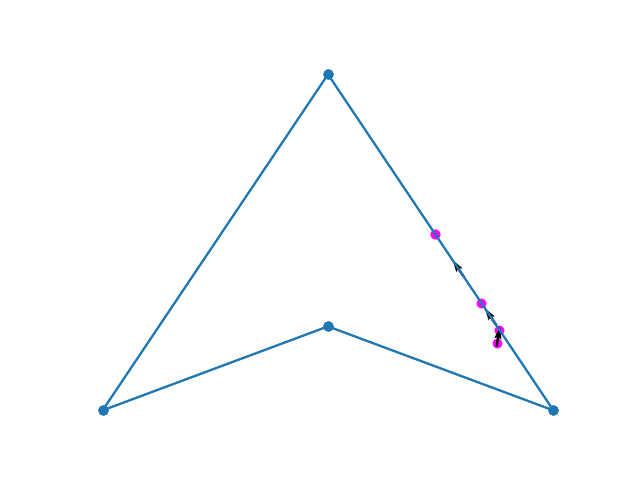
\includegraphics[width = \textwidth]{experiments/concave_triangle_gradient_06.png}
        \caption{Arrowhead polygon gradient with learning rate $\alpha = 0.6$ example.}
        \label{fig:concave_gradient_06}
    \end{subfigure}
    \begin{subfigure}{0.45\textwidth}
        \centering
        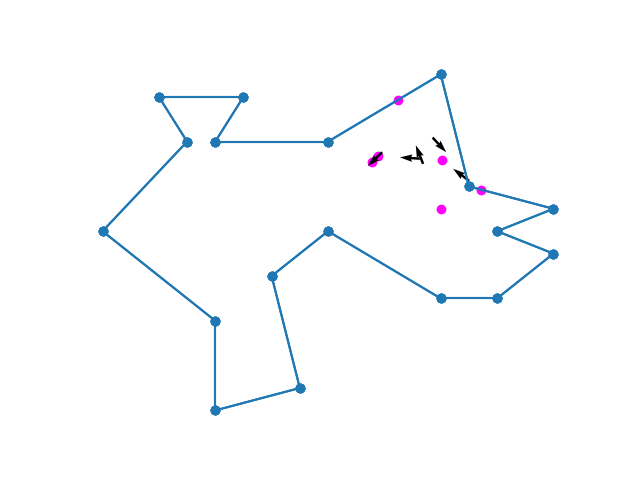
\includegraphics[width = \textwidth]{experiments/random_gradient_045.png}
        \caption{Arbitrary polygon gradient with learning rate $\alpha = 0.45$ example.}
        \label{fig:random_gradient_045}
    \end{subfigure}
    \begin{subfigure}{0.45\textwidth}
        \centering
        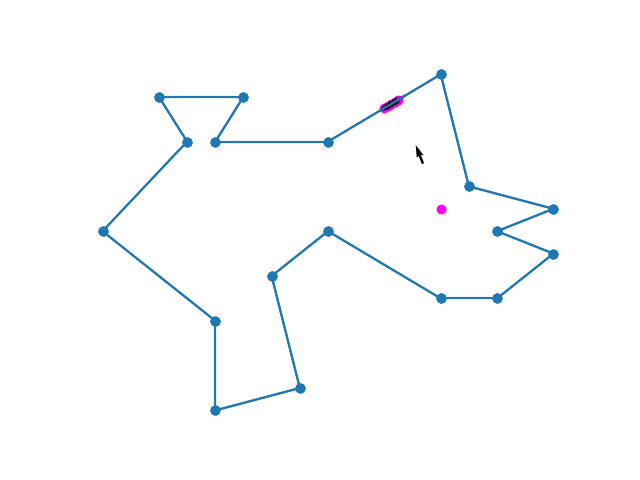
\includegraphics[width = \textwidth]{experiments/random_gradient_06.png}
        \caption{Arbitrary polygon gradient with learning rate $\alpha = 0.6$ example.}
        \label{fig:random_gradient_06}
    \end{subfigure}
    \caption{Gradient descent examples with learning rate $\alpha \in \{0.45, 0.6\}$ on the one-guard Arrowhead and multiple guards arbitrary input polygons.}
    \label{fig:multiple_gradients}
\end{figure}

Subfigures \ref{fig:concave_gradient_045} and \ref{fig:concave_gradient_06} show the transition from $\alpha = 0.45$ to $\alpha = 0.6$, respectively, for the arrowhead polygon. As expected, the steps between the guard positions are bigger. Since only one guard is required to fully view the polygon, the optimum is clearly achieved in both cases. The only major difference between the two learning rates is that when $\alpha$ is larger, less steps are needed to reach the optimum. This behaviour is in accordance to our intuition.

Subfigures \ref{fig:random_gradient_045} and \ref{fig:random_gradient_06} show the transition for the arbitrary polygon from $\alpha = 0.45$ to $\alpha = 0.6$, respectively. Unlike the arrowhead polygon, the arbitrary polygon appears to show a complete opposite evolution. When $\alpha = 0.45$, the guard does not follow a clear path towards an optimum. Instead, it appears that after a few steps it returns to a position close to the starting position. This type of cycling could be accounted for by the gradient computation being unable to escape a local optimum. When $\alpha = 0.6$, we would expect that the guard path is even more chaotic and dispersed. However, the learning rate in this case turns out to be large enough to escape the local optimum that $\alpha = 0.45$ was stuck in. Nonetheless, we expect that even with a larger learning rate, the guard path would still not reach an optimal final position. Because the arbitrary polygon requires multiple guards for full visibility, we predict that the one guard would still be stuck in a cycle between all the guards' local optima.

Therefore, we expect that the choice of the learning rate will be closely intertwined with the type of input polygon and the number of guards required to guard it. This situation will be considered more in-depth in the later phase of this thesis. Then, we can assess whether this is also the case when placing multiple guards.

\subsubsection{Gradient Descent with Momentum}
We have previously observed that one of the drawbacks of gradient descent is that it is computed at every step irrespective of its past values. This can result in sudden irregular changes in the guard's position to optimality. Additionally, it can cause the guard to return to a previously non-optimal computed position, or to remain stuck in local optima. For these reasons, we will extend the computation of gradient descent with momentum \cite{goodfelow2016deep}.

Momentum \cite{goodfelow2016deep} builds upon the idea of considering past states of the gradient descent computation. In this way, the past states act as ``inertia'' to the newly computed gradient state. This results in the overall optimisation trajectory to be smoother. 

There are several methods of implementing momentum in a gradient descent computation. One common approach is to use a moving average. That is, computing the gradient at the current point and then averaging it with the past $m$ values, where $m$ is a hyperparameter. As such, all previous states are given equal weights. Variations of these weights will be observed in the second stage of the thesis.

In these experiments, we will use a moving average of the last 2 gradient descent values. The motivation for choosing this value is related to the total number of steps taken to achieve the optimum in the input polygons. That is, less than 10 steps are taken in total to achieve an optimum within the timeout in the previously discussed experiments. So, we decided to only take into account the last and the second to last position when computing a new one.

\begin{figure}[h!]
    \centering
    \begin{subfigure}{0.45\textwidth}
        \centering
        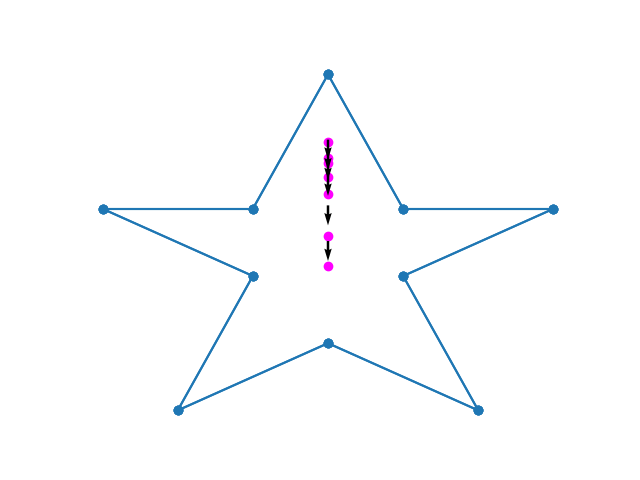
\includegraphics[width = \textwidth]{experiments/pentagram_momentum.png}
        \caption{Star polygon momentum run example.}
        \label{fig:star_momentum}
    \end{subfigure}
    \begin{subfigure}{0.45\textwidth}
        \centering
        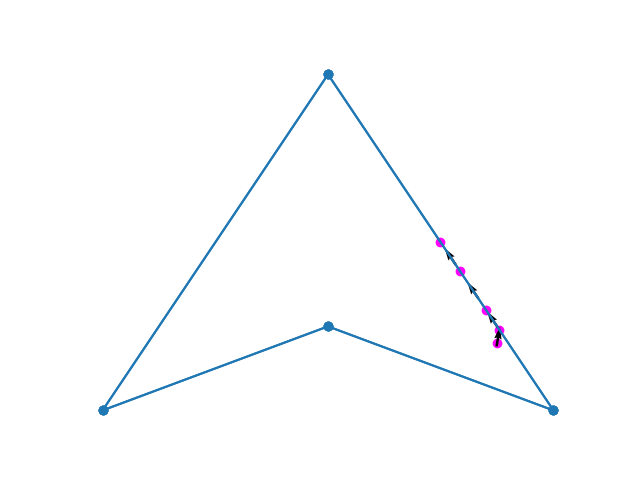
\includegraphics[width = \textwidth]{experiments/concave_triangle_momentum.png}
        \caption{Arrowhead polygon momentum run example.}
        \label{fig:concave_momentum}
    \end{subfigure}
    \begin{subfigure}{0.45\textwidth}
        \centering
        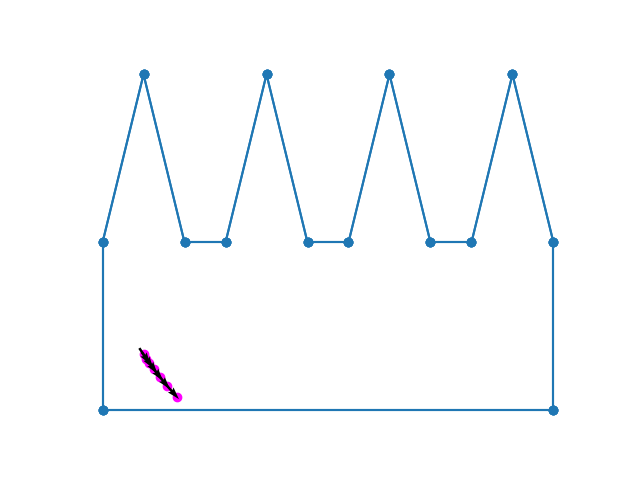
\includegraphics[width = \textwidth]{experiments/comb_momentum.png}
        \caption{Comb polygon momentum run example.}
        \label{fig:comb_momentum}
    \end{subfigure}
    \begin{subfigure}{0.45\textwidth}
        \centering
        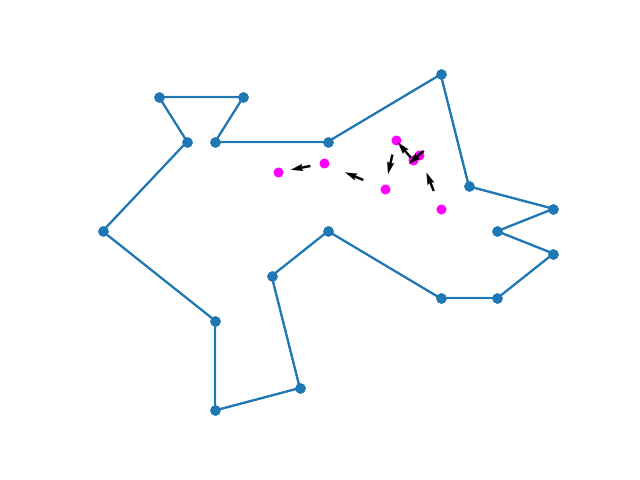
\includegraphics[width = \textwidth]{experiments/random_momentum.png}
        \caption{Arbitrary polygon momentum run example.}
        \label{fig:random_momentum}
    \end{subfigure}
    \begin{subfigure}{\textwidth}
        \centering
        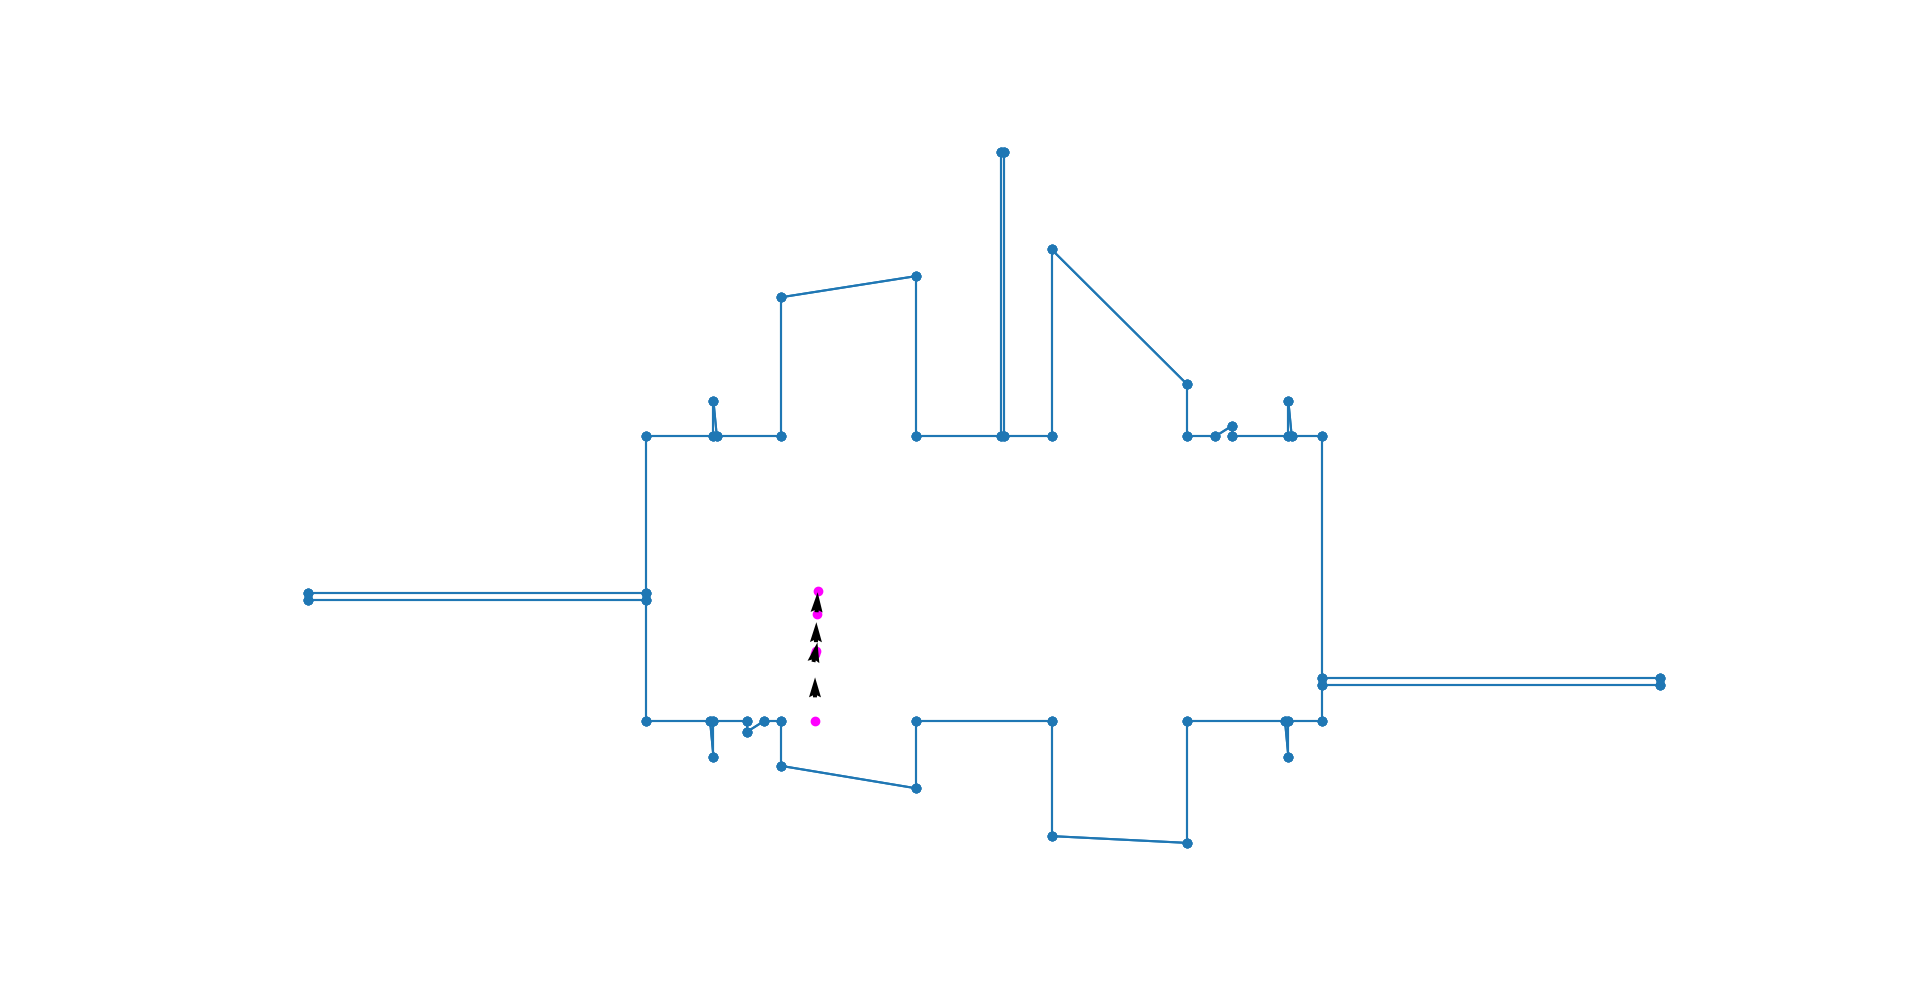
\includegraphics[width = \textwidth]{experiments/love_momentum.png}
        \caption{Irrational guard polygon momentum run example.}
        \label{fig:love_momentum}
    \end{subfigure}
    \caption{Gradient descent with momentum examples with learning rate $\alpha = 0.2$ on the test polygons.}
    \label{fig:momentums}
\end{figure}

Figure \ref{fig:momentums} displays the 1-minute run of the extended algorithm with momentum on the five test polygons. From Subfigures \ref{fig:star_momentum}, \ref{fig:concave_momentum}, \ref{fig:comb_momentum}, and \ref{fig:love_momentum} it becomes clear that the guard's path to optimality is smoothened out. However, these 3 cases do not offer any newer insight than before. On the other hand, Subfigure \ref{fig:random_momentum} confirms that momentum can facilitate the escape of local optima. In this case, the guard manages to escape to the left half of the polygon. This is in contrast to hovering around the local optima on the right half of the polygon.

As such, we claim that expanding the gradient descent computations with momentum would provide a significant improvement to our algorithm. This claim will be quantified more in-depth in the second part of this thesis. 

Therefore, we believe that these experiments found a promising base for the further extension and exploration of them onto the second phase of the thesis.